\section{Results}
\subsection{Analog pixel circuit}
\subsubsection{Values and dimensions}
The transistor technology used limits the width to 

\begin{equation}
    \label{eq:limitsW}
    1.08 \mathrm{\mu m} \leq W \leq 5.04 \mathrm{\mu m}
\end{equation}

and limits the length to

\begin{equation}
    \label{eq:limitsL}
    0.36 \mathrm{\mu m} \leq L \leq 1.08 \mathrm{\mu m}.
\end{equation}

As explained in section \ref{sec:switch_dimensions}, the length and width of the switch transistors will be $1.08\mathrm{\mu m}$.

CS was tuned to $2 \mathrm{pF}$. The output from simulations with this value for the exposure-light corners min-min, min-max, max-min and max-max are shown respectively in figures \ref{fig:min-min}, \ref{fig:min-max}, \ref{fig:max-min} and \ref{fig:max-max}.

\begin{figure}
    \centering
    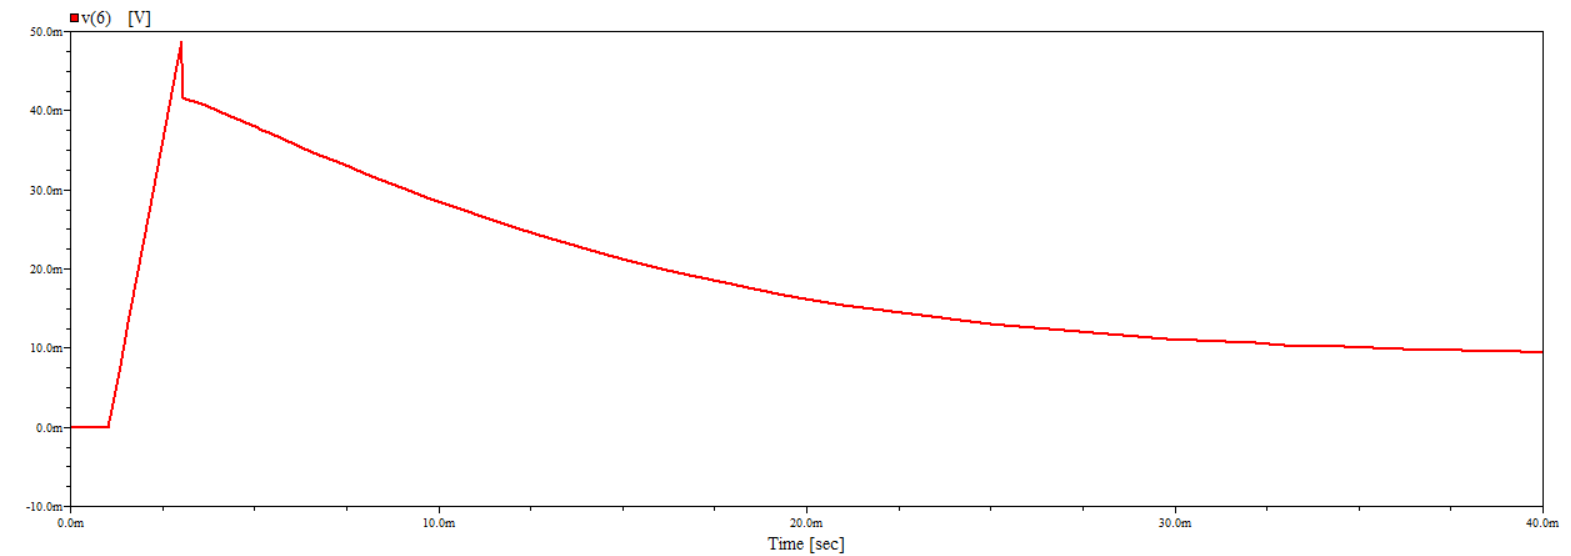
\includegraphics[width=\textwidth]{graphs/minExp_minLight.png}
    \caption{Minimum exposure time - minimum light}
    \label{fig:min-min}
\end{figure}

\begin{figure}
    \centering
    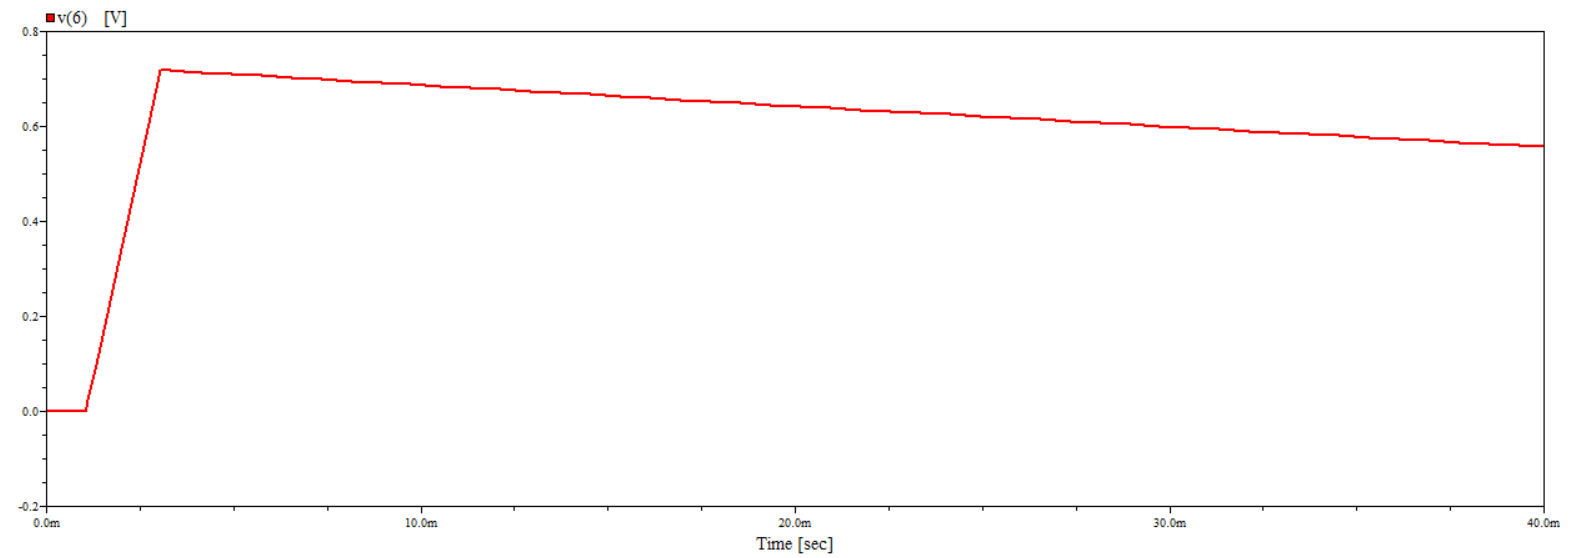
\includegraphics[width=\textwidth]{graphs/minExp_maxLight.png}
    \caption{Minimum exposure time - maximum light}
    \label{fig:min-max}
\end{figure}

\begin{figure}
    \centering
    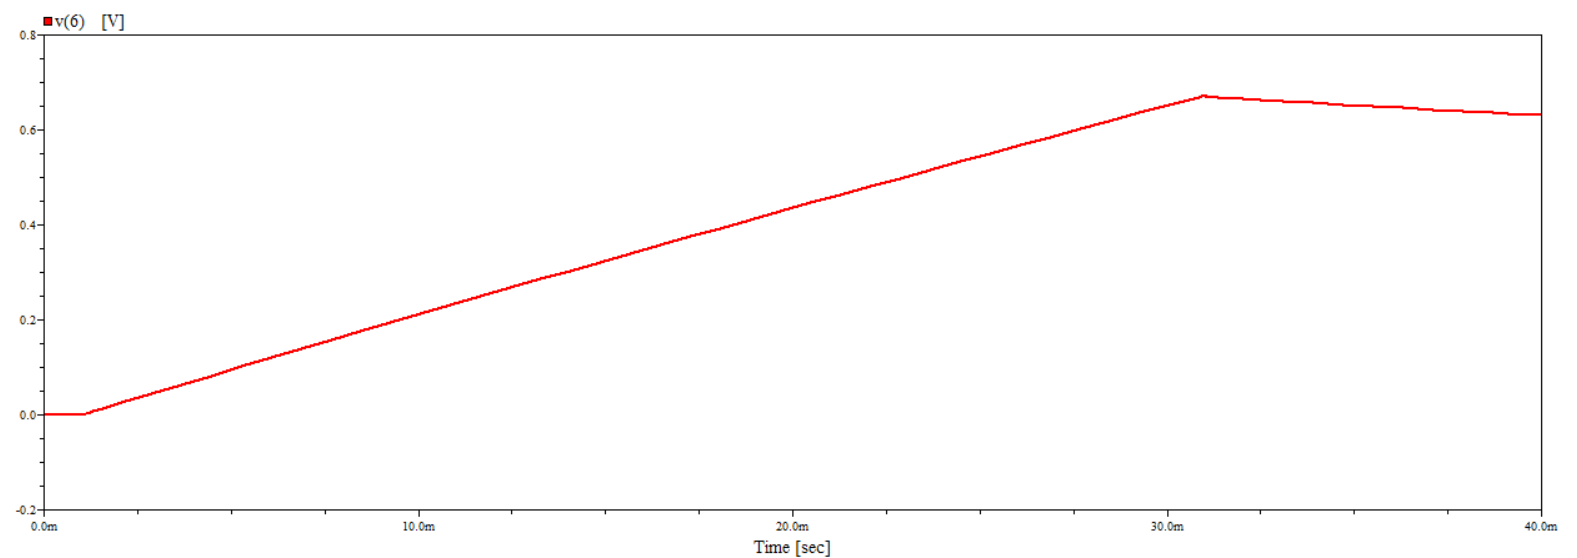
\includegraphics[width=\textwidth]{graphs/maxExp_minLight.png}
    \caption{Maximum exposure time - minimum light}
    \label{fig:max-min}
\end{figure}

\begin{figure}
    \centering
    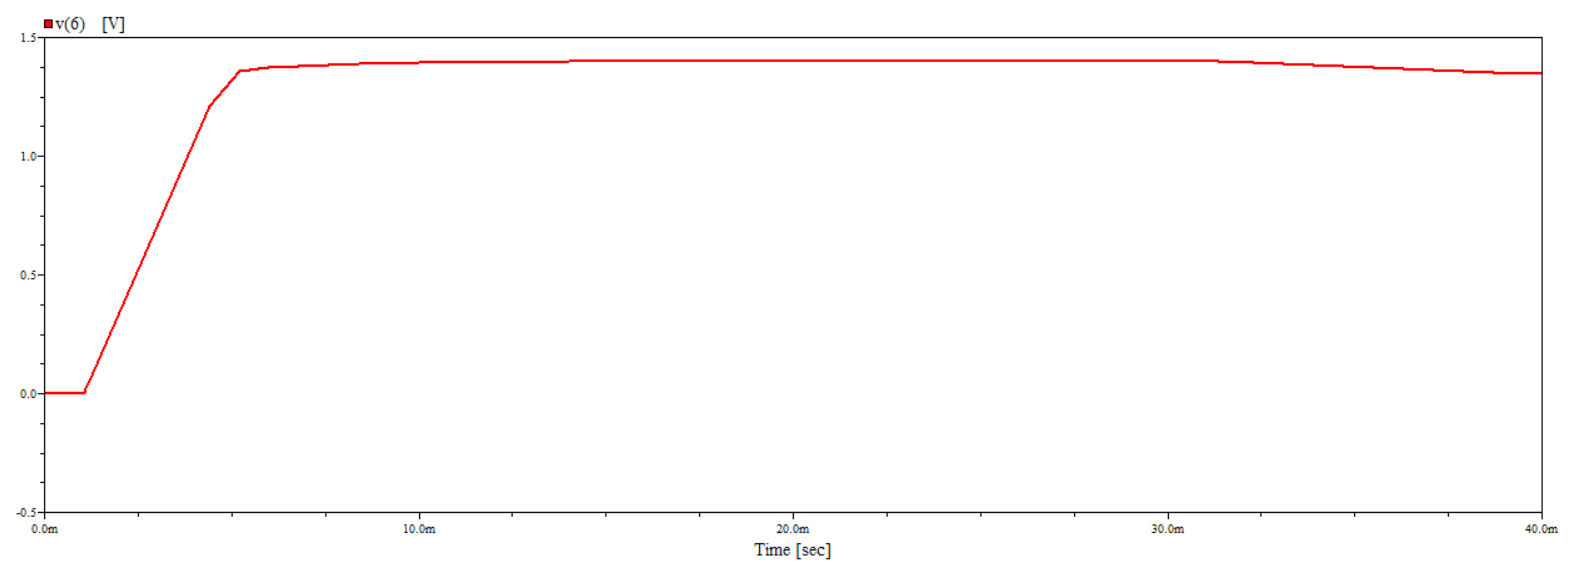
\includegraphics[width=\textwidth]{graphs/maxExp_maxLight.png}
    \caption{Maximum exposure time - maximum light}
    \label{fig:max-max}
\end{figure}

\subsubsection{Analog circuit simulation}

The simulation of the full analog circuit is shown in figure \ref{fig:analogWaveform}. In this simulation the exposure time was $5 \mathrm{ms}$ and the pixels were exposed by photodiode currents of $50 \mathrm{pA}$, $100 \mathrm{pA}$, $300 \mathrm{pA}$ and $750 \mathrm{pA}$.

\begin{figure}
    \centering
    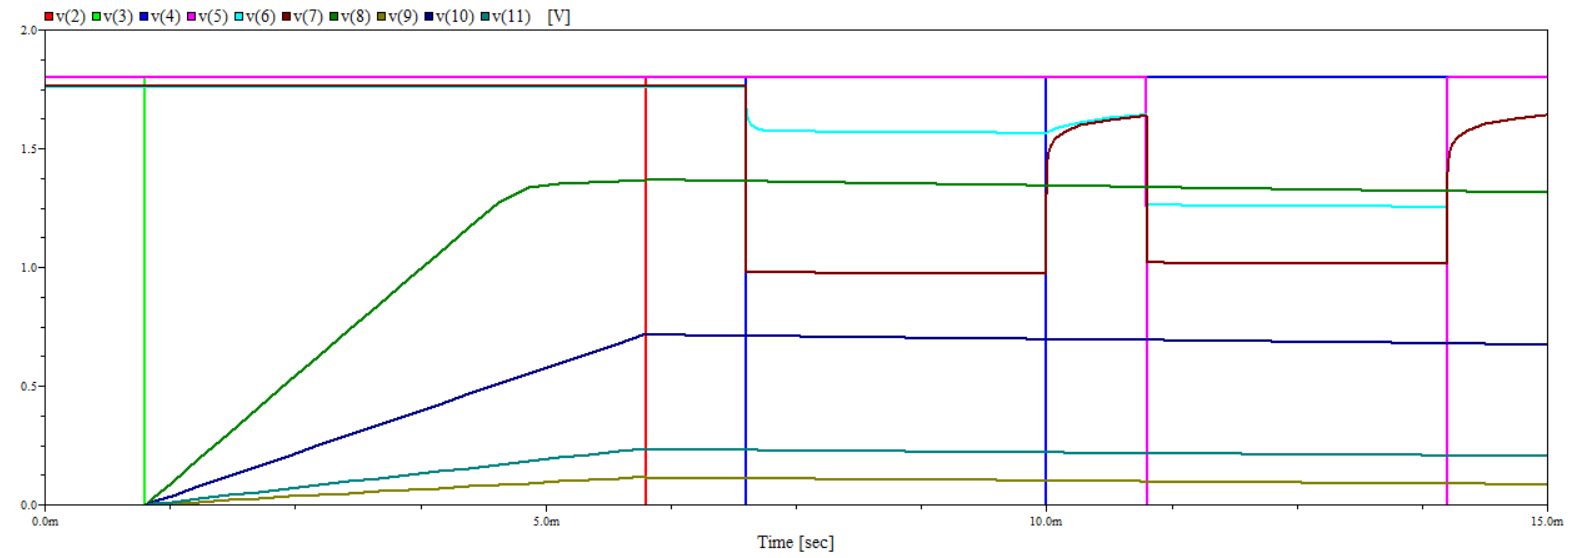
\includegraphics[width=\textwidth]{graphs/analogWaveform.png}
    \caption{Simulation of analog circuit.}
    \label{fig:analogWaveform}
\end{figure}

\subsubsection{Process variation simulations}

\begin{table}
    \centering
    \caption{$R_{DS}$ for an NMOS switch in the fast, typical and slow corners.}
    \label{tab:corners}
    \begin{tabular}{|c|c|c|}
        \hline
        Corner & Off & On \\
        \hline
        FF & $5 \mathrm{G\Omega}$ & $500 \mathrm{k\Omega}$ \\
        TT & $500 \mathrm{G\Omega}$ & $750 \mathrm{k\Omega}$ \\
        SS & $50 \mathrm{T\Omega}$ & $1 \mathrm{M\Omega}$ \\
        \hline
    \end{tabular}
\end{table}

The simulation results for $R_{DS}$ as a function of $V_{GS}$ for a single NMOS are shown in figures \ref{fig:ff}, \ref{fig:tt} and \ref{fig:ss} for FF, TT and SS corners respectively. Table \ref{tab:corners} shows what $R_{DS}$ values this gives when switched fully on and off.

\begin{figure}
    \centering
    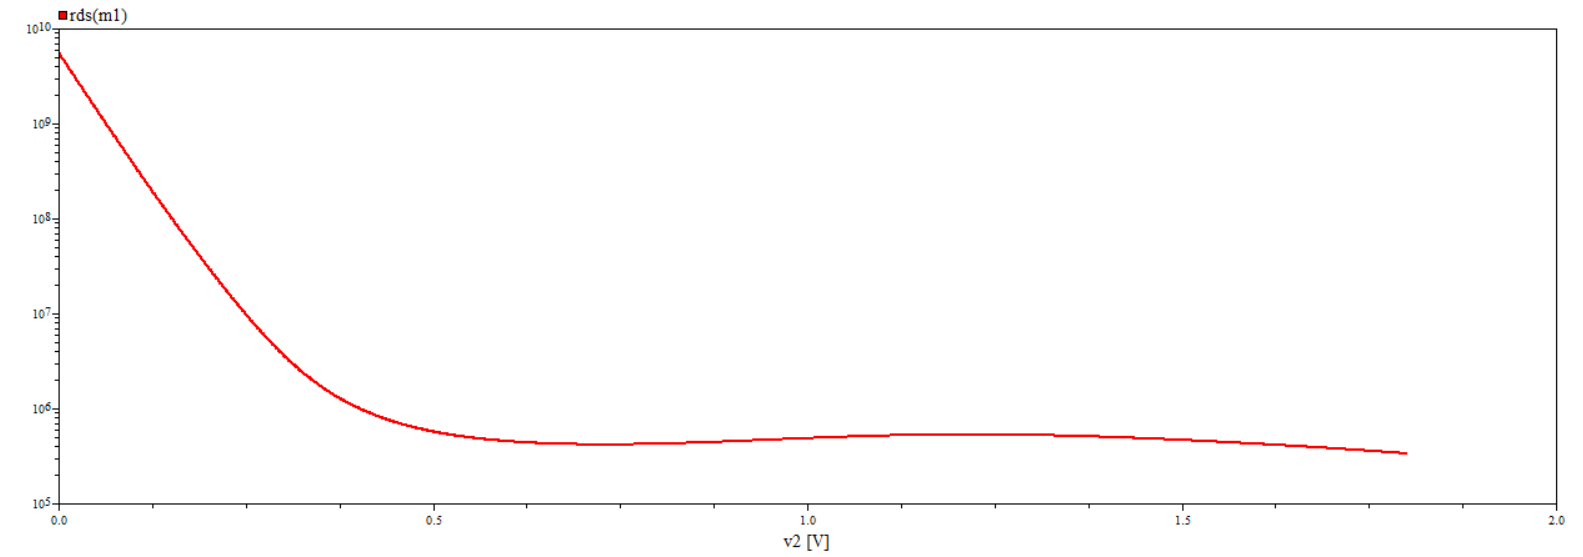
\includegraphics[width=\textwidth]{graphs/corner_ff_simulation.png}
    \caption{FF corner simulation of $R_{DS}$ of NMOS switch as function of $V_{GS}$. $V_{DS} = 1.8\mathrm{V}$.}
    \label{fig:ff}
\end{figure}

\begin{figure}
    \centering
    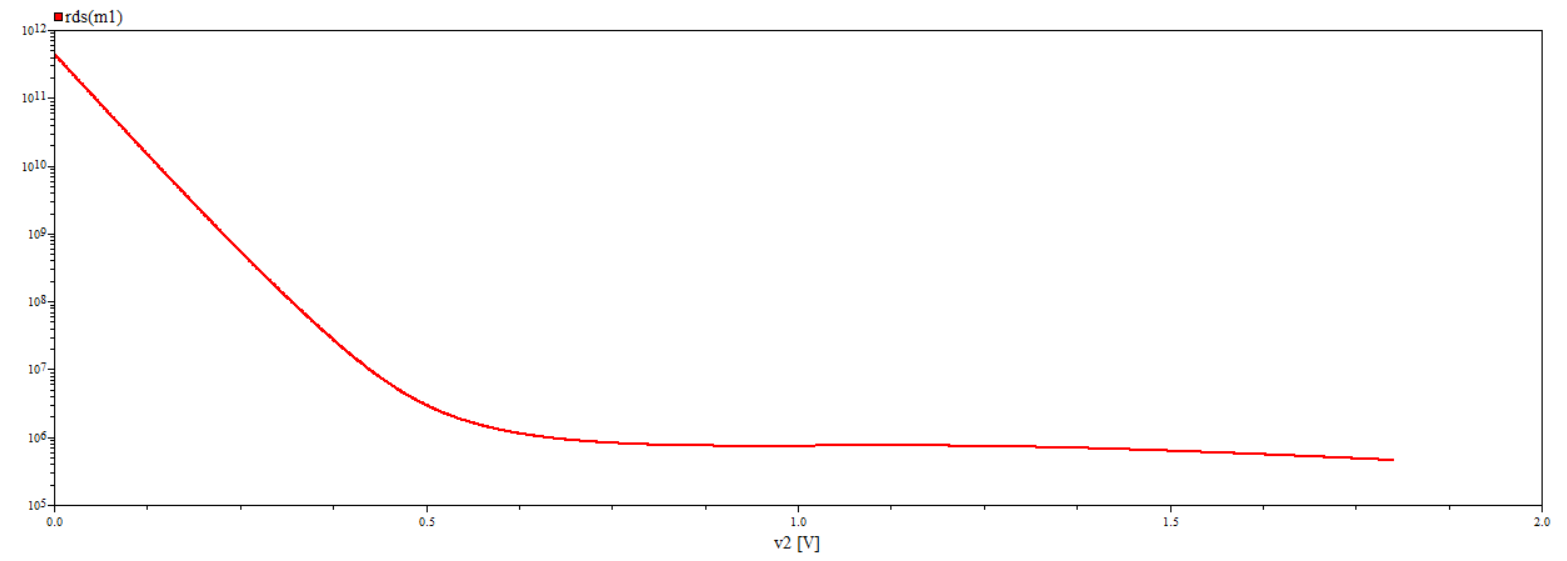
\includegraphics[width=\textwidth]{graphs/corner_tt_simulation.png}
    \caption{TT corner simulation of $R_{DS}$ of NMOS switch as function of $V_{GS}$. $V_{DS} = 1.8\mathrm{V}$.}
    \label{fig:tt}
\end{figure}

\begin{figure}
    \centering
    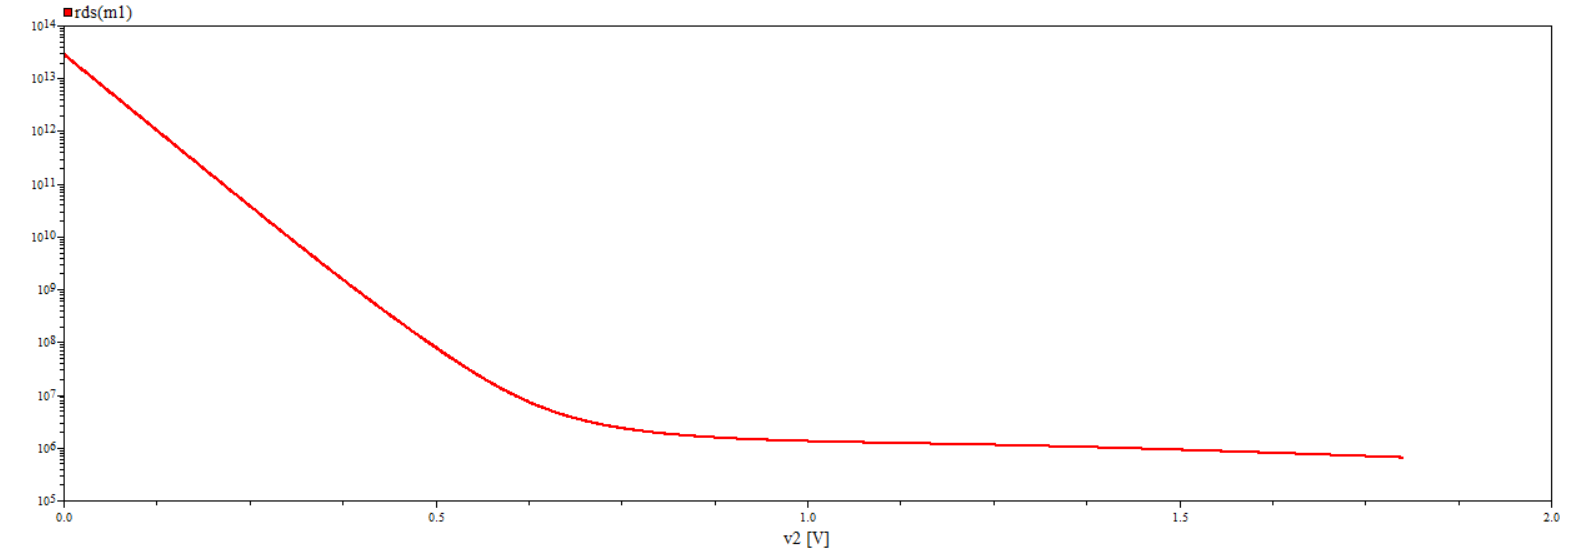
\includegraphics[width=\textwidth]{graphs/corner_ss_simulation.png}
    \caption{SS corner simulation of $R_{DS}$ of NMOS switch as function of $V_{GS}$. $V_{DS} = 1.8\mathrm{V}$.}
    \label{fig:ss}
\end{figure}

Results from full analog circuit simulation in FF and SS corners are shown in figures \ref{fig:ffFull} and \ref{fig:ssFull} respectively.

\begin{figure}
    \centering
    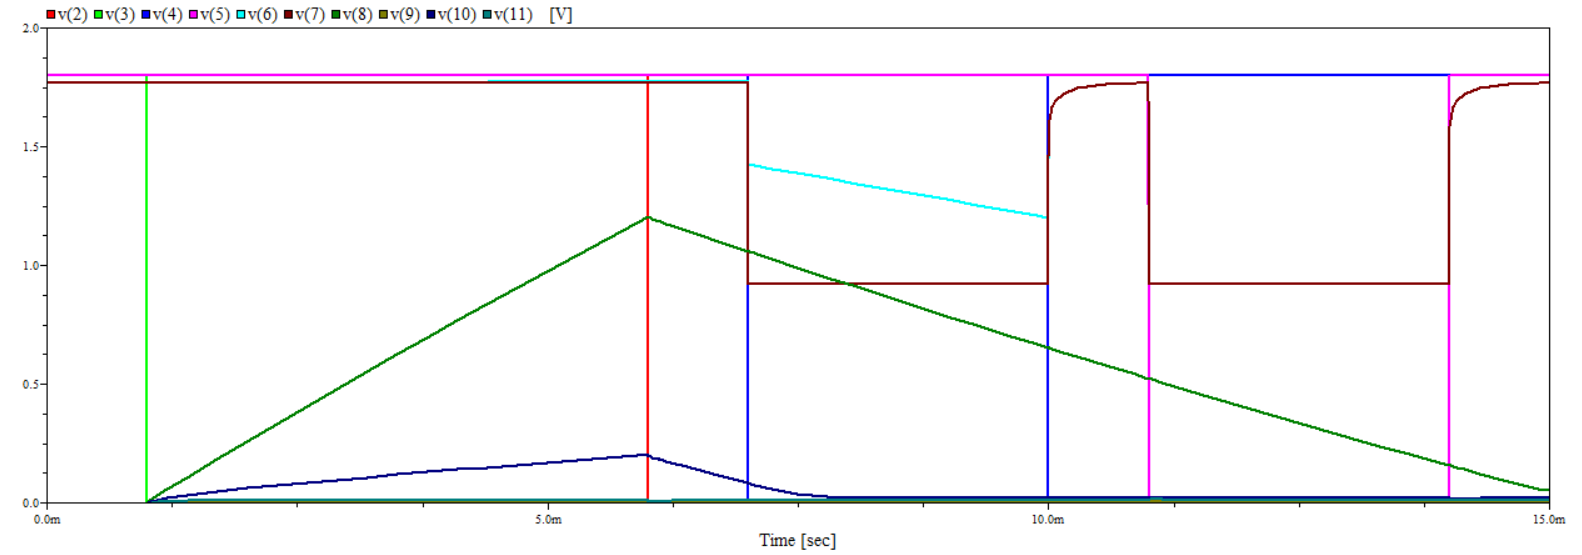
\includegraphics[width=\textwidth]{graphs/analogWaveform_ff.png}
    \caption{FF corner simulation of full analog circuit.}
    \label{fig:ffFull}
\end{figure}

\begin{figure}
    \centering
    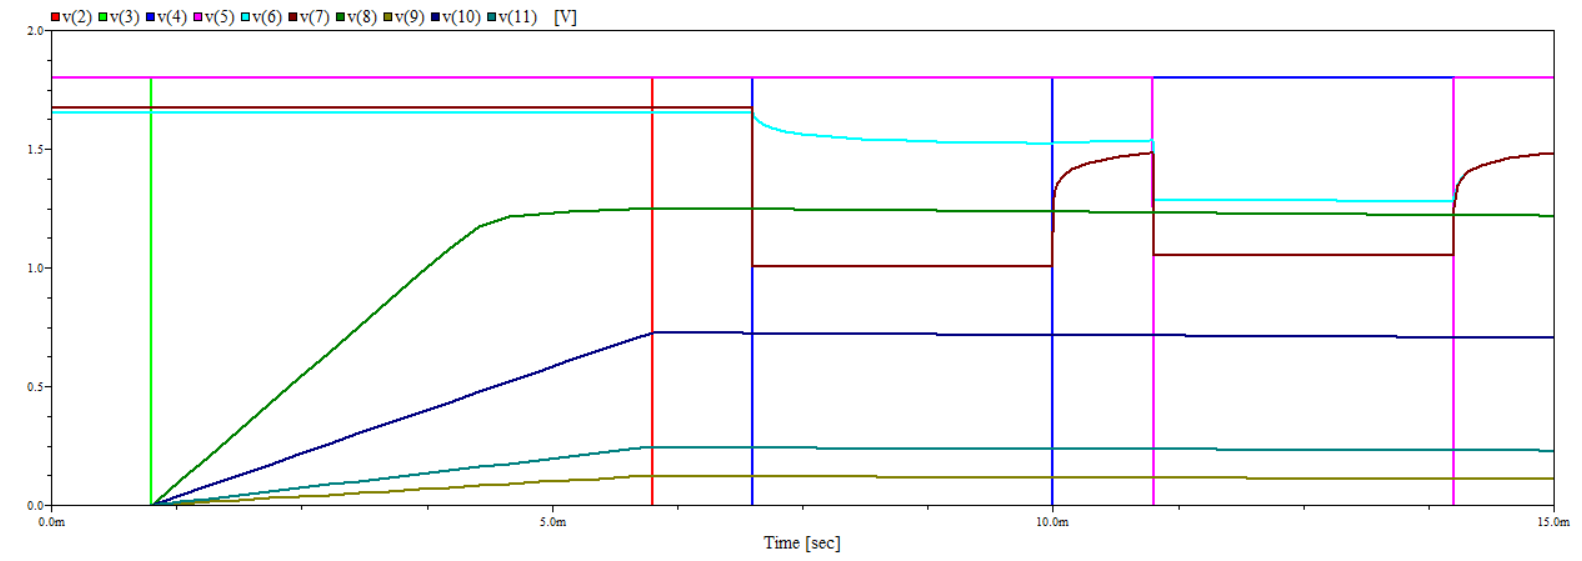
\includegraphics[width=\textwidth]{graphs/analogWaveform_ss.png}
    \caption{SS corner simulation of full analog circuit.}
    \label{fig:ssFull}
\end{figure}

\subsection{Digital circuit}

\subsubsection{Digital circuit simulation}

Explaining the big waveform.

\begin{figure}
    \centering
    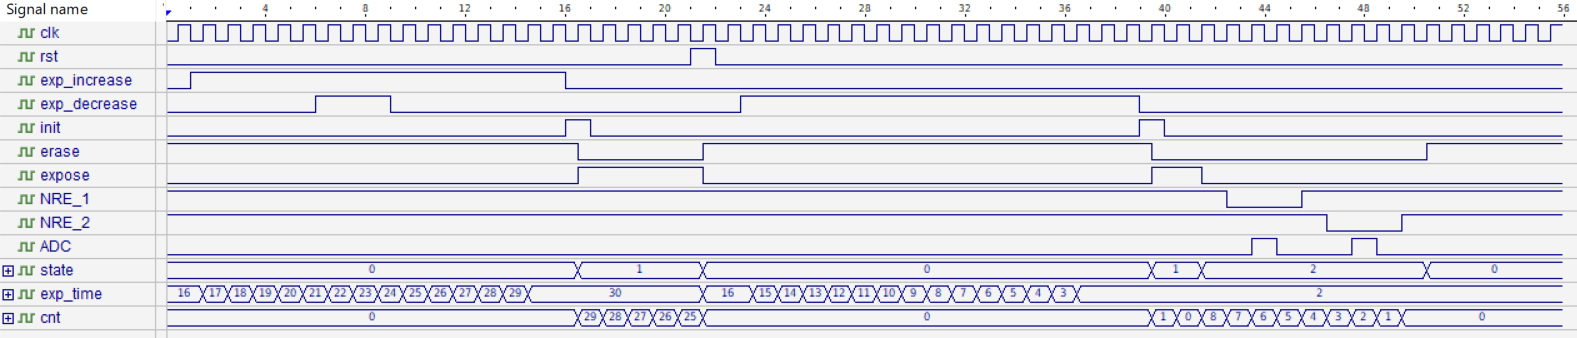
\includegraphics[width=\textwidth]{graphs/digital_waveform.png}
\end{figure}
